\documentclass[tikz,border=10pt]{standalone}

\begin{document}
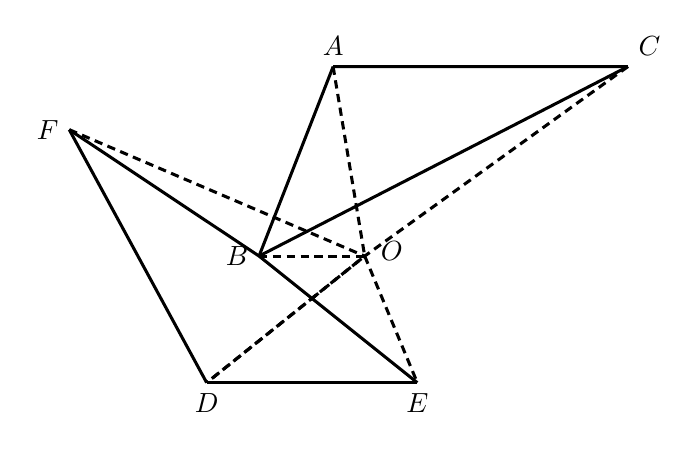
\begin{tikzpicture}[line join=round, line width=1.1pt,
  every node/.style={font=\fontsize{10}{12}\selectfont}]
\coordinate (A) at (-0.206,2.016);
\coordinate (C) at (3.538,2.017);
\coordinate (D) at (-1.812,-1.998);
\coordinate (F) at (-3.557,1.215);








\coordinate (B) at (-1.147,-0.390);
\coordinate (E) at (0.863,-1.998);
\coordinate (P3) at (0.088,0.246);
\coordinate (P4) at (0.195,-0.390);
\coordinate (O) at (0.195,-0.390);
\coordinate (P8) at (-0.418,-0.882);
\coordinate (P10) at (-0.476,-0.929);
\coordinate (P11) at (-0.952,0.097);


\draw (A) -- (C);
\draw (D) -- (E);
\draw (F) -- (D);
\draw (A) -- (B);
\draw (B) -- (C);
\draw (F) -- (B) -- (E);


\draw[dash pattern=on 3pt off 2pt] (A) -- (O);
\draw[dash pattern=on 3pt off 2pt] (C) -- (O) -- (D);
\draw[dash pattern=on 3pt off 2pt] (F) -- (O);
\draw[dash pattern=on 3pt off 2pt] (B) -- (O);
\draw[dash pattern=on 3pt off 2pt] (O) -- (E);
\draw[dash pattern=on 3pt off 2pt] (P8) -- (D);
\draw[dash pattern=on 3pt off 2pt] (P10) -- (O);


\node[above] at (A) {$A$};
\node[above right] at (C) {$C$};
\node[left] at (F) {$F$};
\node[left] at (B) {$B$};
\node[below] at (D) {$D$};
\node[below] at (E) {$E$};


\node[right, xshift=2pt, yshift=2pt] at (O) {$O$};
\end{tikzpicture}
\end{document}